\documentclass{article}
\usepackage[utf8]{inputenc}

\usepackage{url}
\usepackage{geometry}
\geometry{
    a4paper,
    left=20mm,
    top=25mm,
    bottom=25mm,
    right=20mm,
 }
 \usepackage{graphicx}
 \usepackage{titling}
 \usepackage{minted}
 \usepackage{algorithm}
 \usepackage{algpseudocode}

 \usepackage{amsmath}
 \usepackage{amssymb}
 \usepackage{hyperref}
 \usepackage{xcolor}
 % Color of the university of tübingen
 \definecolor{ekut}{RGB}{165, 30, 55}
 \usepackage[printonlyused,withpage]{acronym} % Acronyms with \ac{NCBI} and \acro{NCBI}{National ...}

% Fancy block quotes
\usepackage{mdframed}
\mdfdefinestyle{bquote}{
    linecolor=gray,
    linewidth=1pt,
    leftmargin=20pt,
    innerleftmargin=5pt,
    leftline=true,
    topline=false,
    bottomline=false,
    rightline=false,
    }
\newcommand{\blockquote}[1]{  \begin{mdframed}[style=bquote]  #1  \end{mdframed}}


% BibLaTex / Biber
\usepackage[backend=biber,
    style=numeric,
    uniquelist=false,
    sorting=none,
    url = true,
    isbn = false,
    giveninits=true,
    uniquename=false,
    maxbibnames=6,
    maxcitenames=2,
    minbibnames=5,
    mincitenames=1,
date=year]{biblatex}
\addbibresource{sample.bib}


% No ident for whole document
\setlength\parindent{0pt}

\title{Deep Deterministic Policy Gradients\\Teaching a robot how to walk}
\author{Jules Kreuer, Roman Machacek, Jonas Müller}
\date{\today}

\usepackage{fancyhdr}

\renewcommand{\headrule}{\hbox to\headwidth{
\color{ekut}\leaders\hrule height \headrulewidth\hfill}}

\fancypagestyle{plain}{%  the preset of fancyhdr
    \fancyhf{} % clear all header and footer fields
    \fancyfoot[R]{
\includegraphics[height=1cm]{figures/unilogo.pdf} \hspace{0.2cm} 
\includegraphics[height=1cm]{figures/uio-logo.png}}
    \fancyfoot[C]{\thepage}
    \fancyfoot[L]{May 2023}
    \fancyhead[L]{DDPG - Teaching a robot how to walk}
    \fancyhead[R]{\theauthor}
}
%\pagestyle{plain} % Comment this in if the header / footer should only be on every page.

\makeatletter
\def\@maketitle{%
  \newpage
  \null
  \vskip 1em%
  \begin{center}%
  \let \footnote \thanks
    {\LARGE \@title \par}%
    \vskip 1em%
    %{\large \@date}%
  \end{center}%
  \par
  \vskip 1em}
\makeatother

\usepackage{cmbright}
\begin{document}

\maketitle
\noindent\begin{tabular}{ll}
Author: & Jules Kreuer, Roman Machacek, Jonas Müller\\
Contact: & jules.kreuer@student.uni-tuebingen.de\\
Date of submission: & May 08, 2023\\
Project available on: & \href{https://github.com/not-a-feature/deepq-rl-continuous-control/}{Github}
\end{tabular}
\section{Introduction}\label{sec: Intro}
The paper of \cite{lillicrap2015continuous} proposes a deep reinforcement learning algorithm called Deep Deterministic Policy Gradient (DDPG) for continuous control tasks in robotics and games. DDPG is an actor-critic method that uses two deep neural networks to learn the actor policy and critic Q-function. It is a model-free algorithm that uses off-policy data and is able to handle high-dimensional observation spaces. The authors demonstrate the effectiveness of DDPG on a variety of simulated robotics tasks, including block stacking, cartpole balancing, and humanoid locomotion. They also compare the performance of DDPG to other state-of-the-art methods and show that it achieves better results in terms of both learning speed and final performance.

The proposed method is first presented and then expanded with two new contributions trying to improve reward gaines in the optimization process of the proposed reinforcement learning pipline.

\section{Preliminaries}\label{sec: ...}
Consider an Markov Decision Process $<S, A, R, P>$, with state space $S$, action space $A$, reward function $R$ and state transition function $P$.
\newline
Return is defined as a cumulative reward discounted by $\gamma$: $R = \sum_{t=0}^\infty{\gamma^t r_t}$, where $\gamma \in [0, 1)$.
\newline
Agent actions are modeled through policy function $\pi: S \longrightarrow A$. \\
Further consider functions $V_\pi: S \longrightarrow \mathbb{R}$ and $Q_\pi: S \times A \longrightarrow \mathbb{R}$ representing expected returns by following policy $\pi$.

\subsection{Actor Critic Approach}
The question then is, how do we find an optimal policy $\pi^*$? For this there are two main approaches: Value and Policy based \cite{sutton2018reinforcement}.
In Value based methods we try to approximate an optimal value functions $V_\pi^*$, $Q_\pi^*$. Therefore we are able to evaluate the quality of the current state ($V_\pi$) or state-action pair ($Q_\pi$) based on which we can update our policy $\pi$. Typical example is Q-learning and it's neural network version DQN. Disadvantage of using these methods is that they don't work well for large and continuous spaces.
\newline
Policy based methods on the other hand try to find optimal policy directly without using approximations of value functions. We model our policy with neural network parameterised by $\theta$. We then optimise $\pi_\theta$ using gradients to maximise reward function. Advantage is that we can then use the policy $\pi_\theta$ for continuous spaces and for modelling probability distributions over actions. Main problem with this approach is typically high variance of the policy-gradients, consequently leading to slow convergence and efficiency.
\newline
What if we could combine both approaches? By learning the value function together with policy we could for example reduce gradient variance and improve the convergence.
\begin{enumerate}
    \item Critic: Updates value function parameters
    \item Actor: Updates policy function parameters based on critic
\end{enumerate}

Actor–critic methods are the natural extension of the idea of gradient-based learning methods to temporal difference (TD) learning. TD learning is an technique used to predict an expected reward value in a sequence of states. Instead of calculating total future reward it uses TD error to predict the reward. TD error $\delta_t$ describes the difference between the optimal $V^*$ and predicted value $V$ at step $t$:
\begin{align}
    \delta_t &= V^*(S_{t}) - V(S_t) \\
    \delta_t &= R_{t+1} + \gamma V(S_{t+1}) - V(S_t)
\end{align}
Using this error we can update our value estimation by: $V(S_t) = V(S_t) + \alpha \delta_t$, where $\alpha$ is a hyper-parameter.
\newline
Let's now use state-action values $Q(s, a)$ and look at the reinforcement learning problem from the perspective of neural network parameter optimization.\\
We can use the TD error as a loss function $L$ in order to optimize actor ($\mu$) and critic ($Q$) neural networks, given by the following equation:
\begin{align}
    L(Q', Q, \mu', \mu) = \sum_i (y_i - Q(s_i,a_i) | \Theta^Q)^2,
\end{align}
where we use separate target actor ($\mu'$) and critic ($Q'$) networks in order to get to the used\\
target values $y_i = r_t + \gamma Q'(s_{i+1}, \mu'(s_{i+1} | \theta^{\mu'}) | \theta^{Q'})$.

\section{Continuous Control with Deep RL}
\textbf{Algorithm 1: DDPG}
\begin{algorithmic}
    \small
\State Randomly initialise critic network $Q(s, a|\theta^Q)$ \\and actor $\mu(s|\theta^\mu)$ with weights $\theta^Q$ and $\theta^\mu$.
\State Initialise target network $Q'$ and $\mu'$ with weights $\theta^{Q'} \leftarrow \theta^Q$, $\theta^{\mu'} \leftarrow \theta^\mu$.
\State Initialise replay buffer $R$.\\
\For{episode $= 1, M$}
\State Initialise a random process $N$ for action exploration.
\State Receive initial observation state $s_1$.
\For{$t = 1, T$}
\State Select action $a_t = \mu(s_t|\theta^\mu) + N_t$ according to
\State the current policy and exploration noise.
\State Execute action $a_t$ and observe reward $r_t$ and observe new state $s_{t+1}$.
\State Store transition $(s_t, a_t, r_t, s_{t+1})$ in $R$.
\State Sample a random minibatch of $N$ transitions $(s_i, a_i, r_i, s_{i+1})$ from $R$.
\State Set $y_i = r_i + \gamma Q'(s_{i+1}, \mu'(s_{i+1}|\theta^{\mu'})|\theta^{Q'})$.\\
\State Update critic by minimising the loss: $L = \frac{1}{N}\sum_i(y_i - Q(s_i, a_i|\theta^Q))^2$.\\
\State Update the actor policy using the sampled policy gradient:
\State $\nabla_{\theta^\mu} J \approx \frac{1}{N}\sum_i \nabla_a Q(s, a|\theta^Q)|{s=s_i,a=\mu(s_i)}\nabla_{\theta^\mu} \mu(s|\theta^\mu)|_{s_i}$.\\
\State Update the target networks: \
\State $\theta^{Q'} \leftarrow \tau \theta^Q + (1 - \tau) \theta^{Q'}$ \
\State $\theta^{\mu'} \leftarrow \tau \theta^\mu + (1 - \tau) \theta^{\mu'}$.
\EndFor
\EndFor
\end{algorithmic}

\subsection{Experiments}
The authors tested the DDPG algorithm on a multitude of different reinforcement learning problems (Figure \ref{fig:1})
\begin{figure}[H]

	\centering
	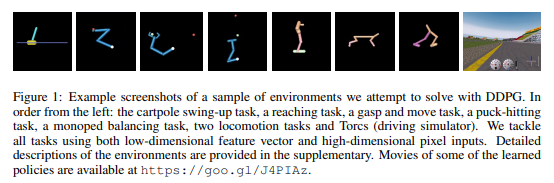
\includegraphics[scale = 0.6]{figures/results_1.png}\hfill

	%\caption{}
	\label{fig:1}

\end{figure}
The researchers tested their algorithm in a variety of simulated physical environments, including classic reinforcement learning tasks like cartpole and high-dimensional tasks like gripper (Figure \ref{fig:1}). They ran experiments using both low-dimensional state descriptions and high-dimensional renderings of the environment. Performance was evaluated periodically during training by testing the policy without exploration noise.

DDPG's performance across all environments was measured, with results averaged over 5 replica. This method was able to learn good policies on many tasks, and in some cases, it learned policies superior to previous known methods.

The algorithm's value estimates were examined by comparing the estimated values after training with the true returns seen on test episodes. In simple tasks, DDPG estimated returns accurately without systematic biases. For harder tasks, the estimates were worse, but DDPG still learned good policies (Figure \ref{fig:2}). The algorithm showed good performance on all tasks, while the variant with target network and batch normalization in the forward pass of the networks suffered from instability.

\begin{figure}[h]

	\centering
	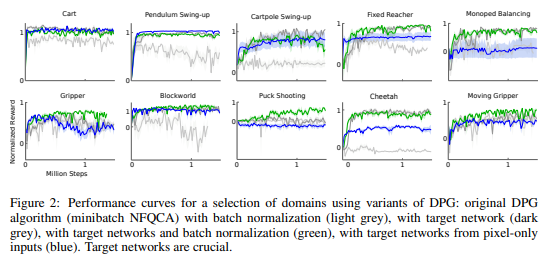
\includegraphics[scale = 0.6]{figures/results_2.png}\hfill

	%\caption{}
	\label{fig:2}

\end{figure}


\subsection{Own Contributions}
Two strategies were investigated to enhance the performance of the algorithm. Given that the algorithm samples random elements from the buffer, we sought to optimize it using two approaches. Initially, we computed a distribution across the elements in the buffer, which subsequently allowed us to sample the buffer according to the distribution weights. The weights are determined by the following equation:

\begin{equation}
    p_i = softmax(\lvert r_i - \mu_R    \rvert),
\end{equation}
where $r_i \in R$ is the reward for element i in the buffer, $\mu_R$ is the mean of the rewards and $softmax$ is the softmax function with temperature parameter $\beta$ given by:
\begin{equation}
    softmax(z_i) = \frac{e^{z_i/\beta}}{\sum_{j=1}^ne^{z_j/\beta}},
\end{equation}
Therefore replay elements are sampled based on their absolute deviation from the mean of the rewards. The underlying idea is that larger deviations correspond to more informative experiences, which are then sampled with greater frequency. The $\beta$ parameter controls the magnitude of the influence of the sampling process, where $\beta$ controls the smoothness of the distribution as the distribution becomes more uniform with increasing $\beta$ and more concentrated at different elements towards 0. Because of the sampling of the buffer with a given distribution we also maintain exploration in the training loop.  \\

In the second method, we employed two distinct buffers derived from the complete replay buffer. The concept involves adding episodes exceeding a specific return threshold $t$ to the "good" buffer, while those falling below are allocated to the "bad" buffer. The threshold parameter is updated dynamically according to the agent's experiences, as shown in the following equation:

\begin{equation}
t_{i} = \mu_{i, \text{roll}} + x * \sigma_{i, \text{roll}}
\end{equation}

In this equation, the new threshold is determined by adding the mean $\mu_{\text{roll}}$ to $x$ times the standard deviation of rewards $\sigma_{\text{roll}}$ from the last 50 episodes. We utilised $x \in {-0.5, 0.5}$ during our experiments. This approach aims to leverage the variability of experiences to perform upper and lower confidence bound weighted sampling of the replay buffer. During sampling, priority can be given either to trajectories from the good or from the bad buffer. This allows to tune the composition of the mini-batch from which the networks learn. We used ratios of 0.7 and 0.5 when sampling.


\section{Results and Discussion}
\begin{figure}[h]

	\centering
	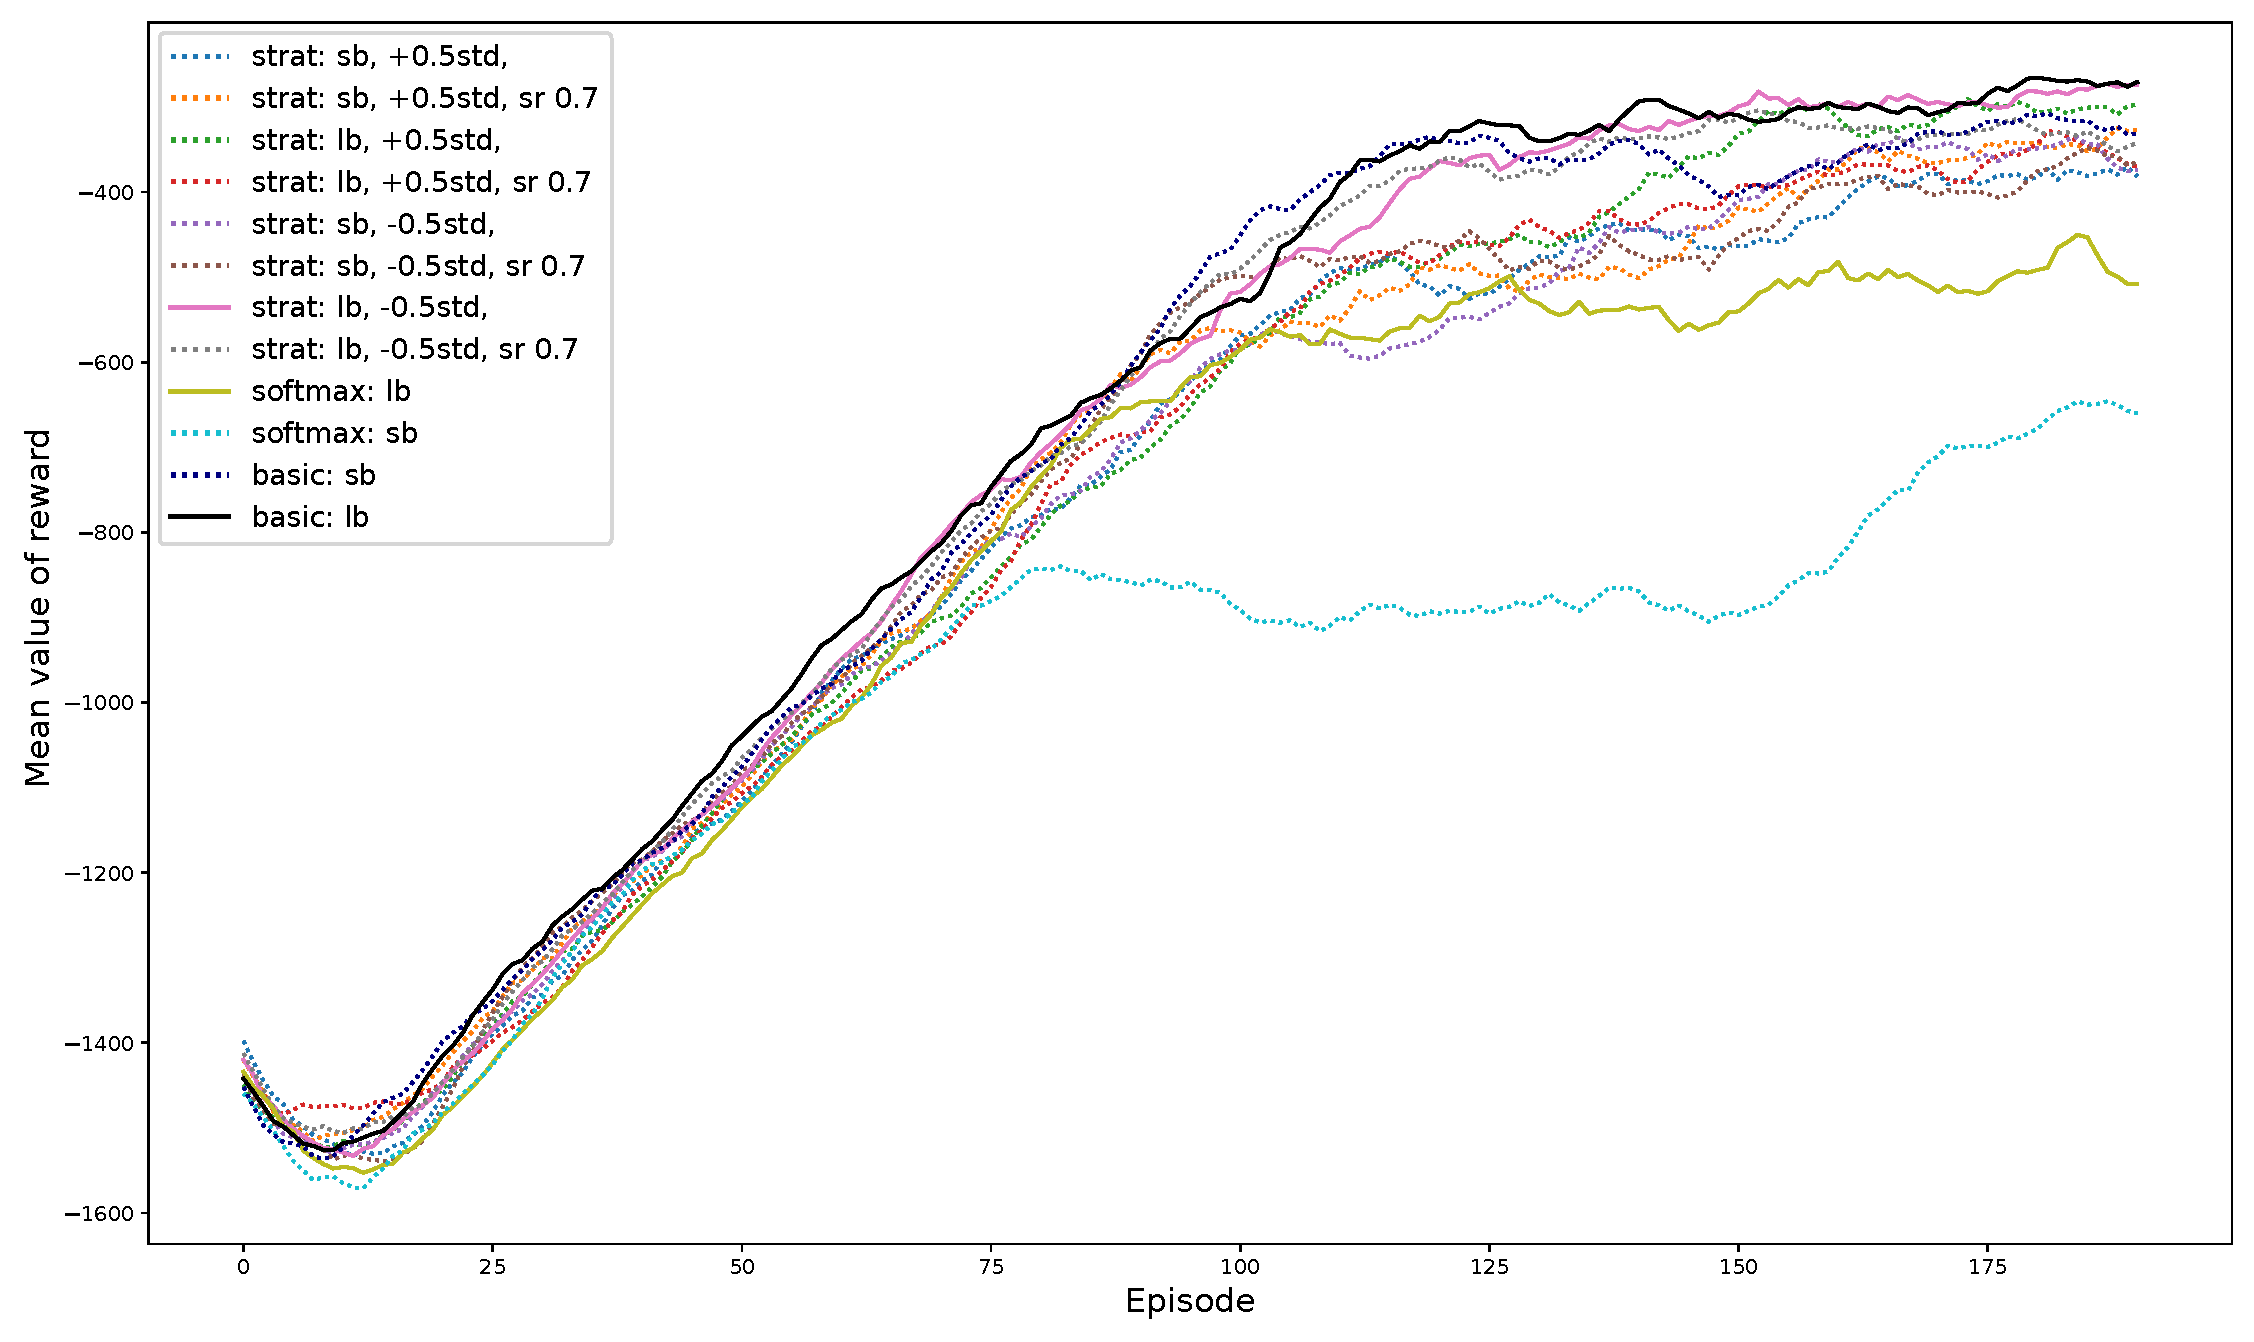
\includegraphics[scale = 0.32]{figures/performance.pdf}
    \caption{Average reward (30 runs, rolling average with window size 10) on Pendulum-v1, all 12 configurations. lb: large buffer ($10^6$), sb: small buffer ($10^4$), sr: sampling ratio of "good" buffer.}
	\label{fig:3}

\end{figure}

In our implementation, we examined two strategies to enhance the performance of the DDPG algorithm: the stratification approach and the softmax method. Both approaches aimed to optimise the sampling process from the replay buffer. However, our results were inconclusive, and we encountered several challenges during the implementation and evaluation of the methods. The reward of 30 runs on Pendulum-v1 with a moving average with window size 10 of all 12 configurations can be seen in Figure \ref{fig:3}).

\subsection{Stratification and Softmax Approach}
The stratification approach carries the risk of the algorithm falling into local maxima depending on the environment's characteristics. For instance, in the BipedalWalker-v3 environment, the agent may become stuck where it remains stationary without falling, avoiding significant penalties. Such a local maxima is not present in the simpler Pendulum-v1 environment where the performance matches the baseline.

The softmax implementation proved to be computationally heavy, taking approximately twice as long to execute compared to the stratification or basic approaches. This increased complexity hindered us from exploring different hyperparameters.

\subsection{Hyperparameter Optimisation}
Both the stratification and softmax methods require hyperparameter optimisation, which adds complexity to the implementation. For example, the performance largely depends on the buffer size, as illustrated in Figure \ref{fig:3}. Here, runs with larger buffer ($10^6$) perform in general better than runs with smaller ($10^4$) ones. Additionally the reward threshold and sampling ratio did impact the performance. The stratification method performed best when using a combination of a large buffer ($10^6$), low threshold ($x = -0.5$) and balanced sampling rate (0.5 / 0.5). This may indicate that episodes with a low reward are still important.

\subsection{Inconclusive Results}
Our inconclusive results can be partially attributed to the small-scale environments and low episode count we used for testing. Due to the computational limitations of a single HPC node, we were unable to thoroughly evaluate the performance of the algorithm on more complex environments.

Interestingly, similar modifications to the buffer were proposed in prioritised experience replay paper \cite{prioritizedreplay}, where they achieved significant improvements using modified importance sampling from the buffer.

\section{Conclusion}

In this study, we reproduced the performance of the training pipeline presented in \cite{lillicrap2015continuous} for the bipedal walker and pendulum tasks. The employed models in addition to the training procedure can be considered as a valuable research avenue for solving continuous control problems with reinforcement learning. In addition we concluded that the proposed replay buffer sampling methods did not yield improvements.
Nonetheless this conclusion shows that the randomness in buffer sampling is necessary to explore the reward space more fully and secure training success without convergence to local minima in the loss landscape.

\printbibliography

\end{document}